%____________________________________________________________________________
%
%STRUTTURA RELAZIONE:
%
%istituto
%scopo
%introduzione teorica
%strumentazione
%procedimento     
%dati sperimentali con tab
%elaborazione dati
%conclusione
%
%_____________________________________________________________________________

%NOTA UTILE: se in un testo bisogna inserire qualche dato numerico in riga, senza
%dover ricorrere a \begin{equation}, basta includere cio' che serve dentro a $....$
%esempio: $10k\Omega$ per inserire il dato in Ohm, poichè alcuni caratteri non vengono presi se stanno fuori da un'equazione


\documentclass{article}
\usepackage{amsmath}
\usepackage{setspace}
\usepackage{anysize}
\usepackage{geometry}
\usepackage{epsfig}
\usepackage{graphicx}
\usepackage{xcolor}
\usepackage{caption}
\usepackage{geometry}
\geometry{a4paper, top=3cm, bottom=3cm, left=2.5cm, right=2.5cm, bindingoffset=5mm}
\captionsetup[table]{position=top, labelformat=empty}
%c'è 1 inch di margine a destra e sinistra
%\geometry{margin = 1.25 in}

\title{ Relazione seconda esperienza di laboratorio Fisica 2}
\author{Gruppo A15: Armani Stefano, Cappellaro Nicola, Pasquato Leonardo}
\date{07-11-2022}
\setlength{\parindent}{0cm}

\begin{document}
    %print sezione titolo
    \maketitle
    \rule{\linewidth}{0.1mm}

    \section{Scopo dell'esperienza}
    Lo scopo della seconda esperienza di laboratorio è stato quello di prendere confidenza
    con due dei principali strumenti utilizzabili nello studio di una rete circuitale:
    il generatore di forme d'onda e l'oscilloscopio.\par
    Per comprendere al meglio il loro funzionamento e l'utilizzo, sono stati applicati
    ad un semplice circuito RC, a cui sono state date in ingresso diverse forme d'onda e 
    sono state studiate le risposte della rete a tali ingressi grazie all'oscilloscopio. 
    
    \section{Cenni teorici}
    Per questa esperienza abbiamo bisogno della formula della scarica di un condensatore e la teoria e formule della regressione lineare.
    La formula della scarica di un condensatore è:
    $V_c(t)=V_0 \cdot e^{-\frac{t}{\tau}}$ \par
    La regressione lineare ci viene in aiuto visto la quantità di dati prelevati.
     Nel nostro caso abbiamo prelevato diversi valori della differenza di potenziale in istanti temporali diversi.\par
    Consideriamo quindi la differenza di potenziale e il tempo come un set di dati sperimentali x e y costituito da n campioni ciascuno.\par 
    Per linearizzare l’andamento della carica avremo che $y=a \cdot e^{-\frac{x}{\tau}}$ \par
    ora applichiamo il logaritmo naturale da entrambe le parti ed otteniamo $ln(y)=ln(a)-{\frac{x}{\tau}}$. \par
    Utilizzando le seguenti sostituzioni: 
    $y'=ln(y)$; 
    $a'=ln(a)$; 
    $b=\frac{1}{\tau}$; 
    otteniamo una funzione lineare del tipo: $y'=a'-bx$.
    A questo punto è possibile usare la regressione lineare per trovare le componenti $a'$ e $b$: 
    $b=\frac{n\sum_{i = 1}^{n} ln(y_i)x_i - (\sum_{i = 1}^{n} ln(y_i))(\sum_{i = 1}^{n} x_i) }{n\sum_{i = 1}^{n} x_i^2 - (\sum_{i = 1}^{n} x_i)(\sum_{i = 1}^{n} x_i)}$; 
    $a'=y'_{medio}-bx_{medio}$. \par


    \section{Strumentazione}
    \begin{itemize}
        \item Breadboard con annessi morsetti serrafilo;
        \item Cavi con connettori a banana e onnettori da banco (Jumper);
        \item Resistori di varie misure ($1k\Omega$, $10k\Omega$, $100k\Omega$) e capacitori da $10nF$, $100nF$;
        \item Generatore di forme d'onda Rigol DG1032;
        \item Oscilloscopio Rigol MSO2102A.
    \end{itemize}

    \section{Esperimento}
    
    Durante la prima parte di questa esperienza di laboratorio sono stati illustrati due
    importanti strumenti da banco, ossia il generatore di forme d'onda (onda quadra, sinusoide, impulso) e l'oscilloscopio: in particolare sono stati
    presentati i parametri di un'onda e il metodo per modularli dal generatore: ampiezza, frequenza, fase, offset \par
    Successivamente sono stati applicati questi due strumenti in un semplice circuito RC, composto da
    un resistore e un capacitore in serie, generatore di forme d'onda e oscilloscopio collegato in parallelo
    al capacitore, come in figura.

    %non è chiaro il perchè, ma il !h potrebbe far incazzare latex
    \begin{figure}[!h]
        \begin{center}
            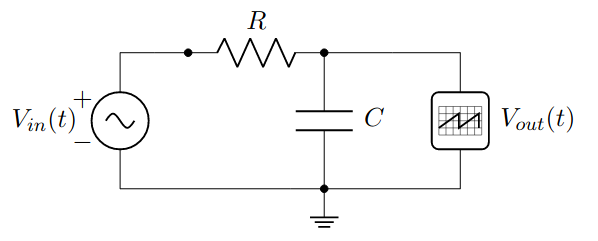
\includegraphics[width = 6 cm]{circuito.png}
            %\caption{Circuito RC}
        \end{center}
    \end{figure}
        
    Il primo esperimento è consistito nel dare in ingresso al circuito, per mezzo del generatore,
    un'onda quadra di frequenza $f = 10Hz$, tensione di picco $V_{In}^{pp} = 5V$ e offset nullo.
    Questo circuito è stato replicato 3 volte, con 3 diverse coppie di resistori e capacitori.
    Grazie all'oscilloscopio è stato possibile ottenere il valore della tensione di lato ai capi 
    del capacitore in funzione del tempo, dunque sono stati ricavati dei valori di tensione istantanea,
    in momenti arbitrari, sia nella fase di carica che di scarica del capacitore.  \par
    Per questioni di semplicità, sono stati utilizzati i valori ottenuti dalla scarica del condensatore, in modo tale
    da poter stimare grazie al metodo della regressione lineare l'andamento della tensione.\par
    Ottenuti i valori delle costanti di tempo caratteristiche per ogni coppia di resistenze e capacità ($\tau$),
    è stato cambiato l'ingresso al circuito: il generatore di forme d'onda è stato impostato in modo tale da generare
    un'onda impulsiva.
    La stessa procedura per ottenere i valori di tensioni istantanee è stata applicata anche in questo caso,
    al fine di studiare l'andamento della tensione avendo in ingresso un'onda impulsiva.
    L'ingresso impulsivo è stato modulato 3 volte, variando la durata dello stesso.    

    \section{Dati sperimentali}

    Primo esperimento:
    \begin{table} [!htb]
        \begin{minipage}{.32\linewidth}
            \caption{$a$: $R = 10k\Omega$,$C = 100nF$}
            \centering
            \begin{tabular}{|c|c|c|}
                \hline
                \textit{Tempo [$\mu s$]} & \textit{Tensione [V]} \\
                \hline
                120 & 4.5 \\
                \hline
                360 & 3.54 \\
                \hline
                960 & 2.56 \\
                \hline
                1160 & 1.54 \\
                \hline
                2160 & 0.54 \\
                \hline
            \end{tabular}
        \end{minipage}
        \begin{minipage}{.32\linewidth}
            \caption{$b$: $R = 10k\Omega$,$C = 10nF$}
            \centering
            \begin{tabular}{|c|c|c|}
                \hline
                \textit{Tempo [$\mu s$]} & \textit{Tensione [V]} \\
                \hline
                32 & 3.54 \\
                \hline
                96 & 1.96 \\
                \hline
                202 & 0.7 \\
                \hline
                302 & 0.28 \\
                \hline
            \end{tabular}
        \end{minipage}
        \begin{minipage}{.32\linewidth}
            \caption{$c$: $R = 200k\Omega$,$C = 5nF$}
            \centering
            \begin{tabular}{|c|c|c|}
                \hline
                \textit{Tempo [$\mu s$]} & \textit{Tensione [V]} \\
                \hline
                100 & 3.69 \\
                \hline
                300 & 2.919 \\
                \hline
                540 & 2.099 \\
                \hline
                980 & 1.263 \\
                \hline
                1860 & 0.459 \\
                \hline
            \end{tabular}
        \end{minipage}
        
    \end{table}

    Secondo esperimento:
    \begin{table} [!htb]
        \begin{minipage}[c]{0.5\textwidth}
            \caption{$2_a$: $R = 10k\Omega$,$C = 100nF$, $d=100\mu s$}
            \centering
            \begin{tabular}{|c|c|}
                \hline
                \textit{Tempo [$\mu s$]} & \textit{Tensione [mV]} \\
                \hline
                20 & 979.4 \\
                \hline
                520 & 581 \\
                \hline
                980 & 381.8 \\
                \hline
                1980 & 149.4 \\
                \hline
            \end{tabular}
        \end{minipage}
        \begin{minipage}[c]{0.5\textwidth}
            \caption{$2_b$: $R = 10k\Omega$,$C = 100nF$, $d=50\mu s$}
            \centering
            \begin{tabular}{|c|c|}
                \hline
                \textit{Tempo [$\mu s$]} & \textit{Tensione [mV]} \\
                \hline
                20 & 514.6 \\
                \hline
                520 & 298.8 \\
                \hline
                1000 & 199.2 \\
                \hline
                1490 & 99.60 \\
                \hline
            \end{tabular}
        \end{minipage}
    \end{table}

    \section{Elaborazione dati}

    \begin{center}
    \begin{tabular}{|c|c|c|c|c|}
        \hline
        \textit{Misura (caso $a$)} & \textit{t[s]} & \textit{ln($V_a$)} & \textit{$t^2$} & \textit{$t[s] \cdot ln(V_a)$} \\
        \hline
        1 & $120 \cdot 10^{-6}$ & $1.5041$ & $1.44 \cdot 10^{-8}$ & $180.489 \cdot 10^{-6}$ \\
        \hline
        2 & $360 \cdot 10^{-6}$ & $1.2641$ & $12.96 \cdot 10^{-8}$ & $455.086 \cdot 10^{-6}$ \\
        \hline
        3 & $960 \cdot 10^{-6}$ & $0.9400$ & $92.16 \cdot 10^{-8}$ & $902.407 \cdot 10^{-6}$ \\
        \hline
        4 & $1160 \cdot 10^{-6}$ & $0.4318$ & $134.56 \cdot 10^{-8}$ & $500.868 \cdot 10^{-6}$ \\
        \hline
        5 & $2160 \cdot 10^{-6}$ & $-0.6162$ & $466.56 \cdot 10^{-8}$ & $-1330.962 \cdot 10^{-6}$ \\
        \hline
        $\varSigma$ & $4760 \cdot 10^{-6}$ & $3.5238$ & $707.68 \cdot 10^{-8}$ & $707.887 \cdot 10^{-6}$ \\
        \hline
        Media & $952 \cdot 10^{-6}$ & $0.7048$ & \multicolumn{2}{c}{} \\
        \hline
    \end{tabular}
    \begin{tabular}{|c|c|c|c|c|}
        \hline
        \textit{Misura (caso $b$)} & \textit{t[s]} & \textit{ln($V_b$)} & \textit{$t^2$} & \textit{$t[s] \cdot ln(V_b)$} \\
        \hline
        1 & $32 \cdot 10^{-6}$ & $1.2641$ & $1.024 \cdot 10^{-9}$ & $40.255206 \cdot 10^{-6}$ \\
        \hline
        2 & $96 \cdot 10^{-6}$ & $0.6729$ & $9.216 \cdot 10^{-9}$ & $64.60267 \cdot 10^{-6}$ \\
        \hline
        3 & $202 \cdot 10^{-6}$ & $-0.3567$ & $4.0804 \cdot 10^{-8}$ & $-72.0483 \cdot 10^{-6}$ \\
        \hline
        4 & $302 \cdot 10^{-6}$ & $-1.2730$ & $9.1204 \cdot 10^{-8}$ & $-384.436 \cdot 10^{-6}$ \\
        \hline
        $\varSigma$ & $632 \cdot 10^{-6}$ & $0.3074$ & $14.2248 \cdot 10^{-8}$ & $-351.429 \cdot 10^{-6}$ \\
        \hline
        Media & $158 \cdot 10^{-6}$ & $0.0769$ & \multicolumn{2}{c}{} \\
        \hline
    \end{tabular}
    \begin{tabular}{|c|c|c|c|c|}
        \hline
        \textit{Misura (caso $c$)} & \textit{t[s]} & \textit{ln($V_c$)} & \textit{$t^2$} & \textit{$t[s] \cdot ln(V_c)$} \\
        \hline
        1 & $100 \cdot 10^{-6}$ & $1.3056$ & $1 \cdot 10^{-8}$ & $130.563 \cdot 10^{-6}$ \\
        \hline
        2 & $300 \cdot 10^{-6}$ & $1.0712$ & $9 \cdot 10^{-8}$ & $321.372 \cdot 10^{-6}$ \\
        \hline
        3 & $540 \cdot 10^{-6}$ & $0.7415$ & $29.16 \cdot 10^{-8}$ & $400.389 \cdot 10^{-6}$ \\
        \hline
        4 & $980 \cdot 10^{-6}$ & $0.2335$ & $96.04 \cdot 10^{-8}$ & $228.82 \cdot 10^{-6}$ \\
        \hline
        5 & $1860 \cdot 10^{-6}$ & $-0.7787$ & $345.96 \cdot 10^{-8}$ & $-1448.391 \cdot 10^{-6}$ \\
        \hline
        $\varSigma$ & $3780 \cdot 10^{-6}$ & $2.5731$ & $481.16 \cdot 10^{-8}$ & $-367.247 \cdot 10^{-6}$ \\
        \hline
        Media & $756 \cdot 10^{-6}$ & $0.5146$ & \multicolumn{2}{c}{} \\
        \hline
    \end{tabular}
    %grafico a
    \begin{equation}
        \begin{split}
            a: \hspace{0.5 cm}\frac{1}{\tau} = \frac{5 \cdot 707.887\cdot10^{-6}V - 3.5238\cdot4760\cdot10^{-6}}{5\cdot707.68\cdot10^{-8} - 4760\cdot10^{-6}\cdot4760\cdot10^{-6}}
            = -1039.876741s^{-1} \longrightarrow \tau_a = -0.00096s
            \\
            ln{V_0} = (ln{V_a})_{medio} - \frac{1}{\tau}\cdot t_{medio} = 0.7048 - (-1039.876741)\cdot952.10^{-6} = 1.69472419 \longrightarrow V_{0a} = 5.445V
        \end{split}
    \end{equation}
    %grafico b
    \begin{equation}
        \begin{split}
            b : \hspace{0.5 cm}\frac{1}{\tau} = \frac{4 \cdot 14.2248\cdot10^{-8}V - 0.3074\cdot632\cdot10^{-6}}{4\cdot14.2248\cdot10^{-8} - 632\cdot10^{-6}\cdot632\cdot10^{-6}}
            = -9435.820s^{-1} \longrightarrow \tau_b = -0.000105979s
            \\
            ln{V_0} = (ln{V_b})_{medio} - \frac{1}{\tau}\cdot t_{medio} = 0.0769 - (-9435.820)\cdot158^{-6} = 1.567717 \longrightarrow V_{0b} = 4.7957V
        \end{split}
    \end{equation}
    %grafico c
    \begin{equation}
        \begin{split}
            c : \hspace{0.5 cm}\frac{1}{\tau} = \frac{5 \cdot 481.16\cdot10^{-8}V - 2.5731\cdot3780\cdot10^{-6}}{5\cdot481.16\cdot10^{-8} - 3780\cdot10^{-6}\cdot3780\cdot10^{-6}}
            = -1183.529085s^{-1} \longrightarrow \tau_c = -0.000844931s
            \\
            ln{V_0} = (ln{V_c})_{medio} - \frac{1}{\tau}\cdot t_{medio} = 0.5146 - (-1183.529)\cdot756^{-6} = 1.40937 \longrightarrow V_{0c} = 4.09337V
        \end{split}
    \end{equation}
    \end{center}

    \begin{figure}[!h]
        \begin{center}
            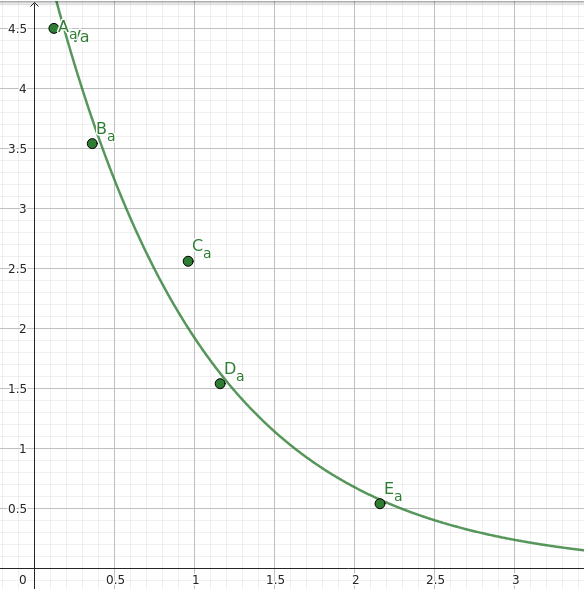
\includegraphics[width = 5cm]{Agraph.png}
            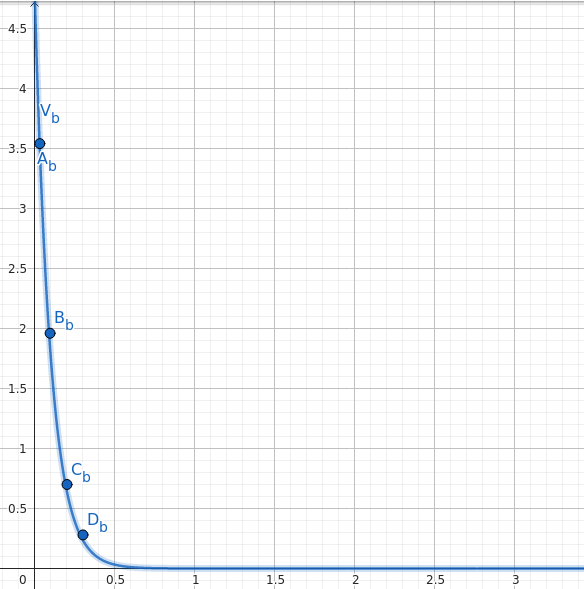
\includegraphics[width = 5cm]{Bgraph.png}
            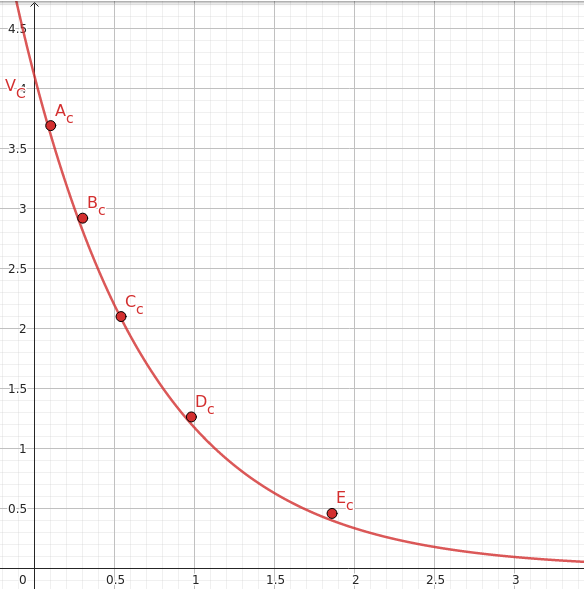
\includegraphics[width = 5cm]{Cgraph.png}
            \caption{Grafici: \color{green}$V_a(t)$, \color{blue}$V_b(t)$, \color{red}$V_c(t)$}
        \end{center}
    \end{figure}

    \newpage
    \section{Conclusione}
    Nel primo esperimento sono state ottenute 3 costanti di tempo ragionevolemte vicine ai valori
    attesi dai calcoli teorici ($\tau = RC$). Solamente il terzo caso, in cui $R = 200k\Omega$ e $C = 5nF$, si discosta maggiormente
    dai valori attesi, soprattutto riguardo l'ampiezza (tensione) d'ingresso e uscita: la tensione picco-picco
    in ingresso risulta essere pari a circa $4 V$, nonostante il generatore crei un'onda quadra di ampiezza
    pari a $5V$. Il motivo è racchiuso all'interno dell'oscilloscopio: utilizzando un'alta resistenza,
    parte della corrente fluisce all'interno della resistenza $R_{osc}$ interna dell'oscilloscopio.\par
    È possibile stimare $R_{osc}$, con $V_{in} = 5V$, $V_{out} \approx 4$: 
    \begin{equation}
        \frac{V_{out}}{V_{in}} = \frac{4V}{5V} = \frac{4}{5} = \frac{R_{osc}}{R_{eq}} = \frac{R_{osc}}{R + R_{osc}} \longrightarrow
        R_{osc} = 4 \cdot R = 4 \cdot 200K\Omega = 800 k\Omega
    \end{equation}
    \par
    Nel secondo esperimento l'onda impulsiva è stata concretizzata da un'onda quadra, di cui è stata modulata la durata a $d_a = 100\mu s$, $d_b = 50 \mu s$, $d_c = 10 \mu s$,
    poichè impulso di ampiezza infinita e durata nulla non è riproducibile nella realtà.
    Il capacitore del circuito RC ha quindi un intervall $d$ di tempo per caricarsi, per poi iniziare a scaricarsi.
    La misurazione manuale diventa allora complicata, poichè minore è l'intervallo $d$ e minore è la carica accumulata dal capacitore.\par
    Per la misurazione della risposta all'impulso del circuito dunque il valore più indicato di $d$ è quello di $d_a = 100 \mu s$.
    Per calcolare la costante di tempo del circuito in risposta all'impulso di durata $d_a$ si prosegue con lo stesso
    procedimento dell'esperimento precedente:
    \begin{equation}
        \frac{1}{\tau} = \frac{-0.0199 - (-0.01197)}{2.06\cdot10^{-5} - 1.22\cdot10^{-5}} = -944.05s^{-1} \longrightarrow \tau = -1.06s
    \end{equation}

    %Nel secondo esperimento invece, l'onda impulsiva è stata concretizzata da un'onda quadra, modulando la sua durata.
    %Tra i 3 tentativi, l'onda quadra che meglio approssima l'impulso è quella con durata minore, anche se la misurazione manuale
    %della tensione diventa complessa.
    
\end{document}